\cut{
1. (way ahead of time) train a statistical model over the training data
2. (at inference time) coarse-grain tokenization (i.e. finding Seqsets)
3a. run the statistical model over the user data, and use the (modified) 
    viterbi algorithm to find the most likely sequences
3b. populate histograms based on the most likely sequences
3c. select candidate histograms + structure, according to heuristics
3d. break down Seqsets using not just the most likely sequences
3e. recursively repeat, go to 3a.
4. apply rewriting involving blob finding to maximize the information 
   theoretic complexity score
5. print description & construct resulting tools

We'll compose this algorithm by figure and explain it with running examples 
in Section 2.
}

\section{Algorithm}\label{sec:algo}

We propose a multi-phase algorithm to attack the problem of
automatically generating tools for ad hoc data. 
The main components of
this algorithm are {\em tokenization} of raw data, 
a top-down, divide-and-conquer {\em structure discovery} procedure,
and a format {\em refinement} phase. This is similar to 
the algorithm proposed in our earlier work \cite{fisher+:dirttoshovels}. 
The key difference is, instead of making definitive decisions about 
tokenizing up front, we defer such decision well into the structure
discovery phase. In particular, we produce {\em all possible} token 
sequences for each data chunk and make choices among these possible 
sequences as the structure is being constructed in an incremental fashion.

\begin{figure}[t]
\begin{centercode}
(1) train a statistical model from the labeled training data;
(2) tokenize the test data into \seqset's, one \seqset{} per chunk;
(3a) find the most probable token sequence for each chunk, and 
     if that sequence of every chunk contains only 1 or 0 edges 
     then return else go to (3b)
(3b) construct histograms from the most probably sequences and 
     predict a top-level structure;
(3c) populate sub-components of the predicated structure with \seqset's
     or sub-\seqset's;
(3d) for each sub-component, recurse to (3a);
(4) apply rewriting rules to improve the overall structure;
(5) print description and generate tools.
\end{centercode}
\caption{High-level Algorithm}\label{fig:algo}
\end{figure}

Fig. \ref{fig:algo} presents this high-level algorithm. We now explain
it step-by-step with the help of {\tt yum.txt} example.
Because this algorithm shares the general structure and many details with
the original algorithm, we only highlight the differences and
refer the reader to \cite{fisher+:dirttoshovels} for complete discussion of
the original algorithm.

\subsection{Training models}
Well ahead of time, a statistical model is trained with
a large pool of sample data formats. Section \ref{sec:stats} has more details
on the various models we attempted in this algorithm. To train the models,
we first label the data using a set of predefined tokens. The set of tokens
used are primarily system oriented, which include
integer, float, time, date, ip address, hostname, file path, URL, 
word, id, white space and punctuations. 
A given substring may be parsed by more than one of the token
types, and we pick a token that best represent the meaning of the data.
We assume that parsing of tokens is {\em greedy}, hence
the string ``43.8'' can be parsed by sequences 
{\tt [int] [.] [int]}, {\tt [int] [.] [float]}, or {\tt [float]},
but not by {\tt [float] [.] [int]} or {\tt [float] [.] [float]},
because the token {\tt float} would parse the entire string, even though
the string ``43'' alone can be represented by a float.

\subsection{Tokenization}
At runtime, each chunk of test data is parsed into a set of all possible 
token sequences. Because these sequences have
common subsequences, we organize them in a directed acyclic graph
called \seqset. Fig.\ref{fig:seqset} shows the \seqset{} after parsing 
the substring ``2.2.13-4'' from a chunk in Fig.\ref{fig:yum}. It 
forms a small part of the \seqset{} from parsing the entire chunk.

\begin{figure}[th]
\begin{center}
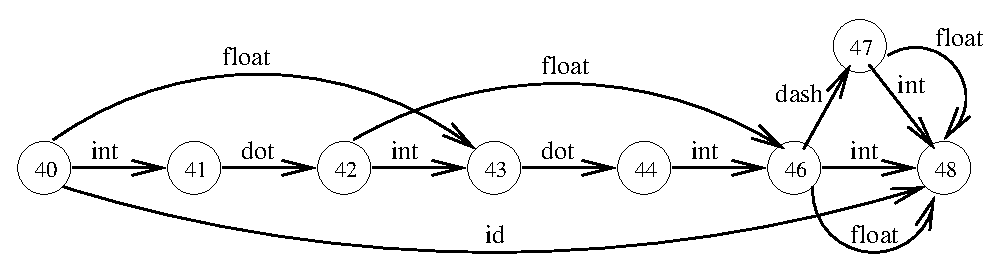
\epsfig{file=seqset.eps, width=0.9\columnwidth}
\end{center}
\caption{\seqset{} from parsing string ``2.2.13-4''}\label{fig:seqset}
\end{figure}

The edges of the \seqset{} are tokens and the vertices are the end locations
of the preceding token. If there is no preceding token (e.g. the leftmost
vertex of the entire \seqset), then the vertex is the begin location 
of first character of next token.
The construction of the \seqset, though expensive, is done only once.
The \seqset{} is used subsequently as input to the recursive 
structure discovery procedure and gets updated during each recursion.

\subsection{Structure discovery}
This is a recursive phase that has several steps.
In (3a), we run the statistical model over the test data
which assigns probabilities to all the edges of the \seqset's.
We then compute the {\em most probable} token sequence, among all alternatives,
for each chunk using a modified {\em Viterbi} algorithm. This algorithm
will be discussed in detail in Section \ref{sec:stats}.
If the most probable sequences contain only 1 or 0 tokens, we have come to
the end of recursion, and return.

Otherwise, in (3b), the histograms are constructed for
all the tokens involved in the most probable token sequences, and we
make a predication of whether the current context is a {\em struct},
{\em union} or {\em array} using the heuristics in \cite{fisher+:dirttoshovels}. 
For example, during the first recursion, 
(3b) would make a prediction that the top level structure of
{\tt yum.txt} is 

{\small 
\begin{verbatim}
struct {date;  ' '; time; ' '; word; ':'; ' '; id; TBD}
\end{verbatim}
}
\noindent
where {\tt TBD} is a context of tokens whose structure is to be determined.

In (3c), \seqset's are modified and populated into the components of
the predicated structure. Suppose at in the next recursion, 
we discover that the {\tt TBD} can be represented by
{\small 
\begin{verbatim}
union{T1; T2}
\end{verbatim}
}
\noindent
where {\tt T1} and {\tt T2} are two sub-contexts 
(whose structures are unknown at this
point) differ by only the first token, 
say {\tt float} vs. {\tt int}. We associate all 
\seqset's whose most likely sequence starts with {\tt float} to {\tt T1} and others with
{\tt T2}. In addition, we break up every \seqset{} in {\tt T1} and {\tt T2} into two sub-contexts:
one that contains just the first token ({\tt float} or {\tt int}) and the other with the rest 
of the tokens.  This amounts to {\em cutting} all the \seqset's into two pieces, 
with the cutting point being the end location of the first token. Edges that are across
the cutting point are removed from the \seqset. Now assume that the statistical
model tells us that the most probable sequence in Fig \ref{fig:seqset} is 
{\small
\begin{verbatim}
[float] [dot] [int] [int]
\end{verbatim}
}
\noindent
then a cut made after the first token will produce two new \seqset's in
Fig \ref{fig:cut}, with the {\tt id}~ edge and the {\tt float} edge between
vertices 42 and 46 removed. \seqset{} on the left will be associated with
the first sub-context and \seqset{} on the right will be associated with the
second sub-context.

\begin{figure}[th]
\begin{center}
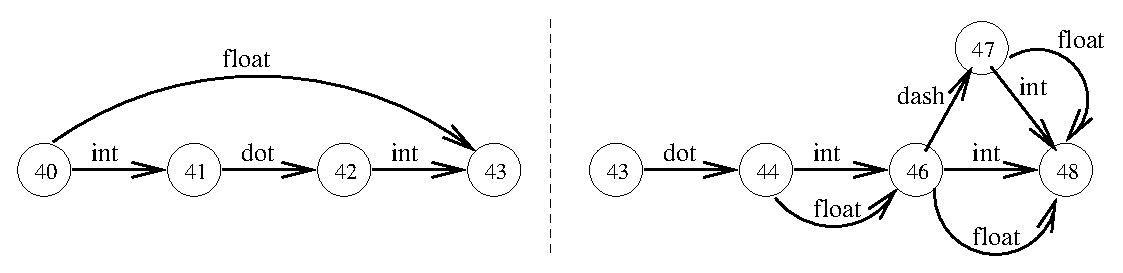
\epsfig{file=cut.eps, width=\columnwidth}
\end{center}
\caption{Cutting a \seqset{} after the first float token} \label{fig:cut}
\end{figure}

If the predicated structure is a struct or an array, similar cuts are
made to all the \seqset's at the boundaries of the contexts.

In step (3d), the procedure recurses to (3a) for each sub-context.

\subsection{Refinement with blob-finding and the rest}
The refinement phase from the original algorithm is augmented with
a ``blob-finding'' step. The purpose of this step is to identify
``message-like'' structures in the intermediate structure and rewrite them into
a single token called {\em blob}, and thus reduce the overall complexity
of the description and increase readability. The blob-finding algorithm
updates the description from bottom up and converts each sub-structure that is
determined to be overly complex and has a terminating pattern into a
blob. The \pads{} parser needs the terminating pattern to
know where the blob ends. Adjacent blobs are merged together. 

A heuristic is used to determine whether a given structure is
a blob. The main idea is to compute a parameter called {\em variance}
for the structure, which measures the total number of union/switch/enum
branches and different array lengths in the given 
structure. When the ratio between the variance and the size of the data
this structure represents exceeds certain threshold, the structure is
determined to be a possible blob. We omit the details of this
heuristic due to space limitations.

After the structure is refined, a \pads{} description is printed out
and a series of tools and libraries can be generated from the description
like in the original algorithm.
